\newpage
\chapter{Background}\label{chap2}
\section{Introduction}
EVT is primarily concerned with the limiting distribution of the maxima or minima of independent, identically distributed (IID) random variables.

Let $X$ be a arbitrary random variable with a cumulative distribution function (CDF) $F$. Moreover, let $X_1,X_2,...,X_n$ be IID random variables. The ordered set is then denoted as $X_{1,n} \leq X_{2,n} \leq...\leq X_{n,n}$. The limit problem is that of finding a potential limiting distributions of the maximum $X_{n,n} = \max(X_1,X_2,...,X_n)$. The distribution of this sample maximum can be written as $P(X_{n,n} \leq x) = F^n(x)$, non trivially for some constants $a_n>0$ and $b_n$: 
\begin{equation}\label{cond1}
F^n(a_n x+b_n) \rightarrow^d G(x), \text{ weakly as } n\rightarrow \infty.
\end{equation}thereby reducing the limit problem to a location and scale problem where $G(x)$ is one of the three possible limiting distribution functions. 

This problem was initially solved by \cite{fisher1928limiting}, and later derived rigorously by \cite{gnedenko1943distribution} and further streamlined by \cite{dehaan1970regular}. The extremal types theorem asserts that if a non-degenerate $G$ exists it must be one of three types:
\begin{eqnarray*}
I&:& \Lambda (x) = \exp\{-e^{-x}\},\ \ \ x\in\mathbb{R}: \\
II&:& \Phi_{\alpha}(x) =
\begin{cases}
 0, & \ x\leq 0 \\
 \exp\{-x^{-\alpha}\}, & \ x>0
\end{cases}
\\&& \text{for some}\ \alpha >0\\
III&:& \Psi(x) =
\begin{cases}
 \exp\{-(-x)^{\alpha}\}, & \ x\leq 0 \\
 1, & \ x>0
\end{cases}
\\&& \text{for some}\ \alpha >0
\end{eqnarray*}
\begin{figure}[h!]
\centering
	\begin{subfigure}[h]{0.49\linewidth}
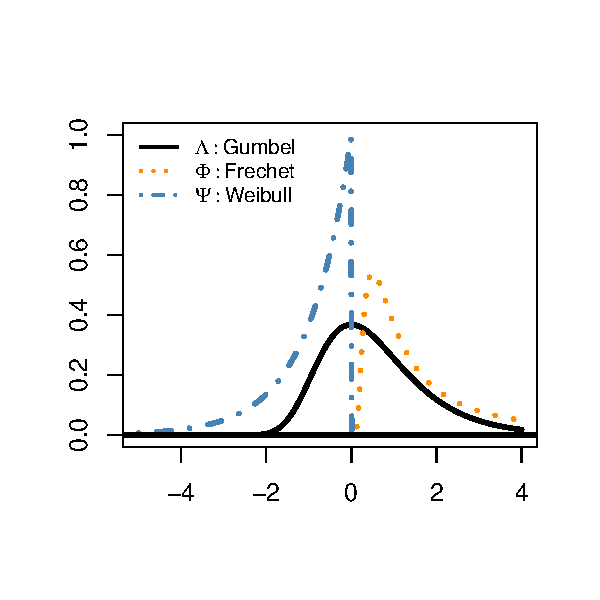
\includegraphics[width=\textwidth]{./plots/chapter2_plots/densities1.pdf}
\end{subfigure}
	%	\hspace{0.1\fill}
			\begin{subfigure}[h]{0.49\linewidth}
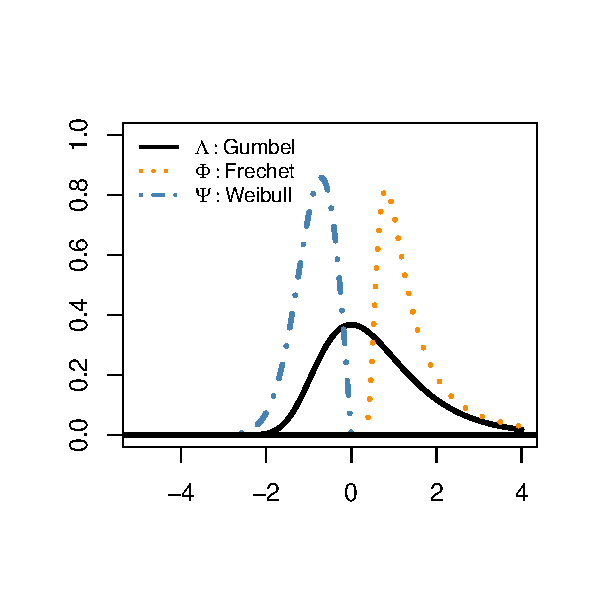
\includegraphics[width=\textwidth]{./plots/chapter2_plots/densities2.pdf}
\end{subfigure}
\caption{Densities of the three standard extreme value distributions. With $\alpha = 1$ (left) and $\alpha = 2$ (right)}
\label{fig:my_label}
\end{figure}

These types of distributions are often referred to as the Gumbel, Fréchet and Weibull types, respectively.
The three types of distributions can be joined into a single distribution function with the following cumulative distribution function (CDF):
\begin{equation}\label{gev1}
G_{\gamma}(x) = 
\begin{cases}
 \exp\left\{ -\left( 1+\gamma x \right)^{-1/\gamma} \right \}, & \text{if}\ \gamma\neq0 \\
 \exp\left\{-e^{-x} \right\}, & \text{if}\ \gamma=0
\end{cases}
\end{equation}defined on $\{x: 1+\gamma x > 0\}$ and $\gamma \in \mathbb{R}$.
This CDF is known as the Generalised Extreme value (GEV) distribution. The parameters $\gamma$ is known as the shape parameter, also known as the EVI. This parameter is of primordial importance in EVT.

\begin{figure}[h!]
\centering
	\begin{subfigure}[h]{0.49\linewidth}
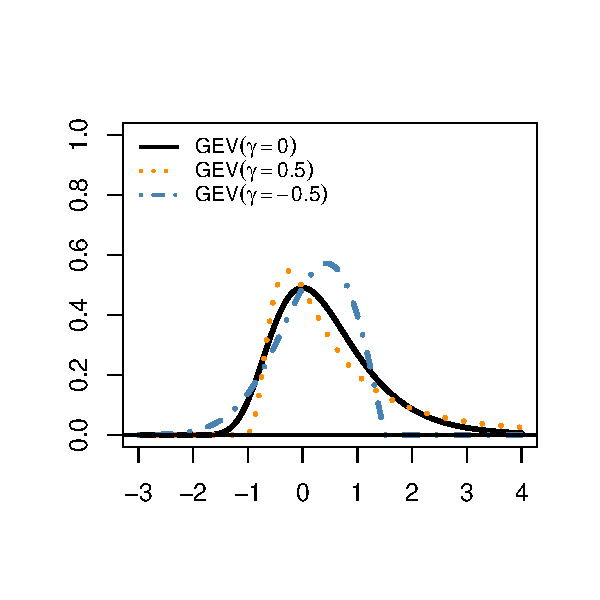
\includegraphics[width=\textwidth]{./plots/chapter2_plots/gevdensity1.pdf}
\end{subfigure}
	%	\hspace{0.1\fill}
			\begin{subfigure}[h]{0.49\linewidth}
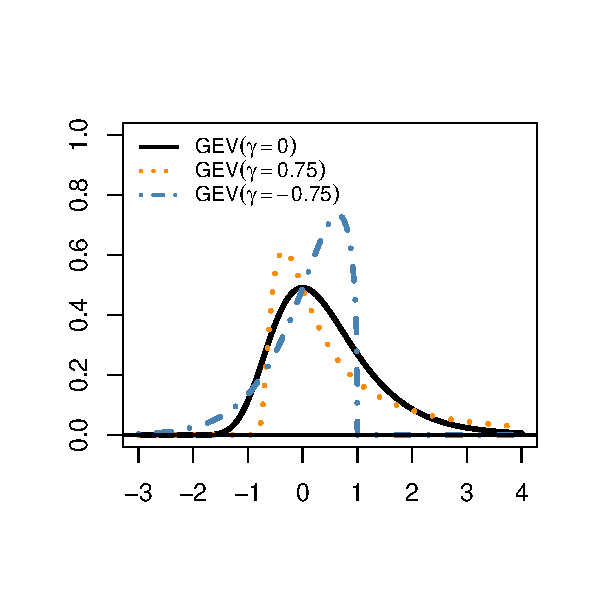
\includegraphics[width=\textwidth]{./plots/chapter2_plots/gevdensity2.pdf}
\end{subfigure}
\caption{Densities of the $GEV(\gamma)$ with $\gamma$ choices: 0,0.5,-0.5 (left) and 0,0.75,-0.75 (right)}
\label{gev}
\end{figure}
It becomes clear from Figure \ref{gev} that the EVI affects the tail behaviour. If $\gamma = 0$, the GEV distribution decays exponentially and belongs to the Gumbel family. If $\gamma > 0$, the GEV distribution has a much heavier tail and belongs to the Fréchet family. Lastly if $\gamma < 0$, the GEV has a finite upper endpoint and belongs to the Weibull family.

If (\ref{cond1}) holds, we can say that the underlying distribution $F$ is in the domain of attraction of $G_{\gamma}$ and write $F\in \mathcal{D}(G_{\gamma})$. This is the set of distributions attracted to $G_{\gamma}$. For example it can be shown that the Loggamma distribution is in the domain of attraction of $G$ with $\gamma > 0$.

The rigorous mathematical framework provided by EVT necessitates some assumptions about regularity conditions for the underlying distributions. Throughout the different parts of this thesis we refer to the well known, necessary and sufficient conditions for $F\in \mathcal{D}(G_{\gamma})$. Without going into much detail we therefore make a brief overview of the necessary and sufficient conditions in order to give a preliminary context.

Define the support of a distribution function $F$ by the lower bound ${}_{+}x := \sup\{x: F(x)=0\}$ and the upper bound $x_+ := \inf\{x: F(x)=1\}$. The quantile function $Q(y)=F^{\leftarrow}(y)=\inf\{x: F(x)\geq y \}$ and the tail quantile function $U(y) = F^{\leftarrow}\left( 1-\dfrac{1}{y} \right)$.
%###########################################################################################################

\subsection*{First-Order Condition}\\
Consider the underlying distribution function $F$ underlying in the extremal domain of attraction of the GEV distribution, $F\in \mathcal{D}(G_{\gamma})$.
There exists a positive measurable function $a$ for which \citep{de1984slow}:
\begin{equation}\label{condition1}
\lim_{t\rightarrow\infty} \dfrac{U(tx)-U(t)}{a(t)} = D(x) =
\begin{cases}
\dfrac{x^{\gamma}-1}{\gamma}\ \ &\text{if } \gamma \neq 0\\
\log(x)\ \ &\text{if } \gamma \neq 0
\end{cases}
\end{equation}for all $x > 0$.

\cite{de1984slow} shows that Equation (\ref{condition1}) is equivalent to the following statement:\\
{\it There is a positive function $a$ such that:}
\begin{equation}\label{condition1b}
\lim_{t\rightarrow\infty} t(1-F(a(t)x + U(t))) = (1+\gamma x)^{-1/\gamma}
\end{equation}{\it for all $x$ with }$1+\gamma x >0$.\\
\hspace*{\fill}$\blacktriangle$

\begin{definition}\textnormal{\textbf{Regular variation}} \\
	All functions ultimately zero are said to belong to a class of regular varying functions if:\begin{equation}
	\lim\limits_{t\rightarrow \infty}\dfrac{f(tx)}{f(t)}=x^{\rho},\ \ \ \text{for}\ x>0, \text{with some } \rho \in \mathbb{R},
	\end{equation}$f$ is said to be regular varying with index $\rho$, $f\in RV_{\rho}$. Furthermore a function $f$ is said to be slowly varying if for $x>0$: \begin{equation}
	\lim\limits_{t\rightarrow \infty}\dfrac{f(tx)}{f(t)}=1.
	\end{equation}
\end{definition}

\subsection*{Second-Order Condition}
\subsubsection*{A general tail ($\gamma\in\mathbb{R}$)}
$F$ satisfies the second order condition if there exists a function $A(t)$, tending to zero as $t\rightarrow\infty$, such that:
\begin{equation}\label{2nd}
\lim\limits_{t\rightarrow\infty}\dfrac{\dfrac{U(tx)-U(t)}{a_0(t)}-\dfrac{x^{\gamma}-1}{\gamma}}{A(t)}=H_{\gamma,\rho}(x):=\dfrac{1}{\rho}\left(\dfrac{x^{\gamma+\rho}-1}{\gamma+\rho}-\dfrac{x^{\gamma}-1}{\gamma}\right)
\end{equation}
for all $x>0$ and $a_0>0$, with $\rho <0$, the second order parameter controlling the speed of convergence of the partial maxima towards the limit law. It is then said that the function $U$ is of second order extended regular variation, and write $U\in 2ERV_{\gamma,\rho}$, noting also that, $|A|\in RV_{\rho}$ and tends to zero, hence larger absolute values of $\rho$ correspond to a higher rate of convergence.

\subsubsection*{A heavy tail ($\gamma>0$)}
In case of heavy tails the second order condition reads as follows. The existence of the function $\tilde{A}(t)$ is such that:
\begin{equation}
\begin{array}{ll}
\lim\limits_{t\rightarrow\infty}\dfrac{\dfrac{U(tx)}{U(t)}-x^{\gamma}}{\tilde{A}(t)}&=x^{\gamma}\dfrac{x^{\tilde{\rho}}-1}{\tilde{\rho}}\Longleftrightarrow\\& \lim\limits_{t\rightarrow\infty}\dfrac{\ln U(tx)-\ln U(t)-\gamma\ln x}{\tilde{A}(t)}=\dfrac{x^{\tilde{\rho}}-1}{\tilde{\rho}}
\end{array}
\end{equation}
for all $x>0$, and $\tilde{\rho}\leq 0$, the second order parameter. As in the general case, we then say $U$ is of second order regular variation and write $U\in 2RV_{\gamma,\tilde{\rho}}$. $F$ is said to satisfy the second order condition \citep{alves2007note}.
\hspace*{\fill}$\blacktriangle$

There is a special class of Pareto type distributions, known as the Hall class. This is a wide class of models containing most useful heavy-tailed parents such as those used in this thesis, namely: the Fréchet and the Burr XII distribution.\\
\begin{definition}\label{hall}\textnormal{\textbf{Hall class of distributions}}\ \\
	Assuming the underlying distribution $F$ satisfies $F(0)=0$, the survival function of a distribution in the Hall class \citep{hall,welsh} can be written as:
	\begin{equation}\label{hallclassF}
		\bar{F}(t)=C^{1/\gamma}t^{-1/\gamma}[1+\gamma^{-1}DC^{\rho/\gamma}t^{-\rho/\gamma}+o(1)],\ \ t\uparrow \infty, 
	\end{equation} where $\gamma >0, C>0, \rho<0$ and $D\in\mathbb{R}$.\\
\end{definition}

For any $\tau=\rho/\gamma$ and $C^{1/\gamma}\propto C$, we can write (\ref{hallclassF}) as:
\begin{equation}\label{F}
	1-F(x)=Cx^{-\alpha}[1+Dx^{\tau}+o(x^\tau)],\ \ \ x\uparrow \infty, 
\end{equation} where $\alpha >0, C>0, \tau<0$ and $D\in\mathbb{R}$.
\autoref{F} can also be written as a tail quantile function: \begin{equation}
	U(t)=Ct^{\gamma}\left(1+\dfrac{A(t)}{\rho}+o(t^{\rho})\right),\ \ \ A(t)=\gamma\tau t^{\rho}.
\end{equation}

Much more insightful readings on second order conditions and regular variation can be found in the famous work of \cite{de1996generalized}. \cite {alves2007note} also 
provides a very comprehensive overview of the first, second and third order conditions. In this thesis we do not make use of this third order frame work. Furthermore a detailed explanation of the characterisation of normalising constants $a_n$ and $b_n$ more specific to the first order condition, can be found in \cite{leadbetter2012extremes}. Table \ref{domain}\footnote{Table \ref{domain} is adapted from \cite{albrecher2017reinsurance}} provides a short list of some of the very common distribution functions classified according to the different domains.

%###########################################################################################################

\begin{table}[h]
\centering
\begin{tabular}{llll} 
\toprule
\textbf{Domain } & \textbf{Distribution } & $1-F(x)$& $({}_{+}x,x_+)$ \\ 
\hline
\multirow{3}{*}{\begin{tabular}[c]{@{}l@{}}Weibull \\$\gamma < 0$ \end{tabular}} & Reversed Burr & $\beta^{\alpha}(\beta+x_{*}-x)^{-\tau})^{-\alpha}$ & $(0,x_{*})$ \\
 & Extreme Weibull& $1-e^{-(1-x)^{\alpha}}$& $(0,x_{*})$ \\
 & Beta& $\dfrac{1}{B(p,q)}\int^1_x u^{p-1}(1-u)^{q-1}$ & $(0,1)$ \\ 
\hline
\multirow{3}{*}{\begin{tabular}[c]{@{}l@{}}Gumbel \\$\gamma = 0$ \end{tabular}} & Gamma & $\dfrac{\lambda^{\alpha}}{\Gamma(\alpha)}\int^{\infty}_x e^{-\lambda u}du$ & ($0,\infty$) \\
 & Exponential& $e^{-\lambda x}$& ($0,\infty$) \\
 & Log Normal & $\int^{\infty}_x \dfrac{1}{\sqrt{2\pi}\sigmat}\exp\left( -\dfrac{1}{2\sigma^2}(\log u-t)^2 \right) du$ & ($0,\infty$) \\ 
\hline
\multirow{3}{*}{\begin{tabular}[c]{@{}l@{}}Fréchet\\$\gamma > 0$ \end{tabular}} & Strict Pareto & $(x/x_0)^{-\alpha}$& $(x_0,\infty)$\\
 & Burr (XII) & $\beta^{\alpha}(\beta+x^{\tau})^{-\alpha}$ & $(0,\infty)$ \\
 & Log-gamma & $\int^{\infty}_x \dfrac{\lambda^{\alpha}}{\gamma(\alpha)} u^{-\lambda - 1} \log(u)^{\alpha-1} du$& $(1,\infty)$ \\
\hline
\end{tabular}
\caption{A list of some common distributions and their respective domains of attraction }
\label{domain}
\end{table}

\section{Motivating data set}\label{mtplsection}
In order to demonstrate the need for EVT and methods proposed in this thesis, a simplified case study in reinsurance is considered. 
\subsection{Reinsurance: Motor Liability Data}
We present in this section a motor third-party liability (MTPL) data set first studied by \cite{albrecher2017reinsurance}.
This data contains 849 insurance European claims between 1995 and 2010 evaluated on 1 January 2011. 59\% of these claims were not closed at the time of evaluation. To account for inflation and reflect costs in the calendar year 2011, all amounts have been indexed.
\\\\
In order to make claim reservations, insurance companies will have experts approximate the ultimate losses still under development alongside aggregate payments and incurred losses. In case a claim is closed during the study period, the ultimate value is then the aggregate payment.
\begin{figure}[h!]
\centering
	\begin{subfigure}[h]{0.49\linewidth}
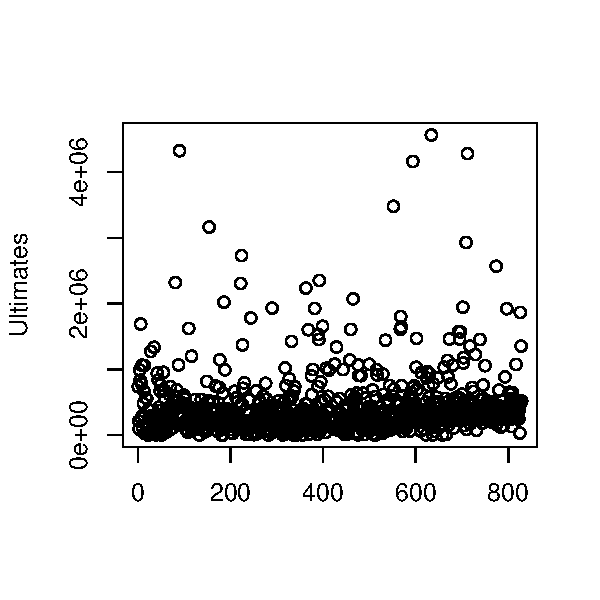
\includegraphics[width=\textwidth]{./plots/chapter2_plots/ultimates.pdf}
\end{subfigure}
	%	\hspace{0.1\fill}
			\begin{subfigure}[h]{0.49\linewidth}
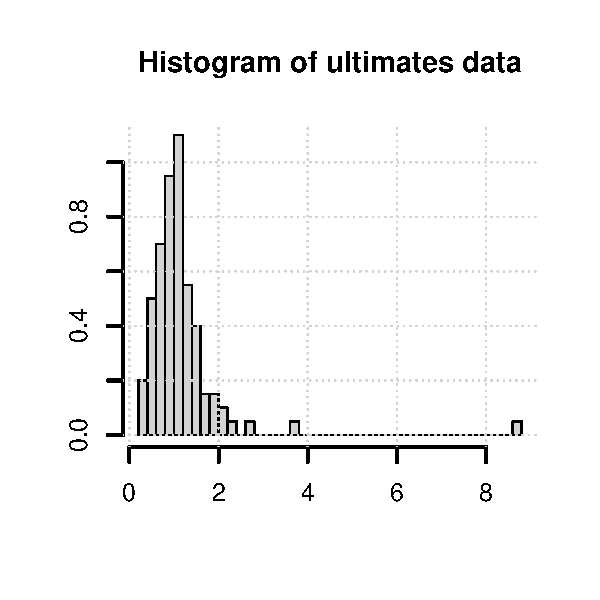
\includegraphics[width=\textwidth]{./plots/chapter2_plots/mtpl_dens.pdf}
\end{subfigure}
\caption{Scatter plot of ultimates loss data (left) and the corresponding empirical density plot (right)}
\label{fig:hist}
\end{figure}
\begin{table}[h]
\centering
\resizebox{\linewidth}{!}{%
\begin{tabular}{llllll} 
\hline
\textbf{min} & \textbf{1st~quartile} & \textbf{median} & \textbf{mean} & \textbf{3rd~quartile} & \textbf{max} \\ 
\hline
90& 167,389& 286,296 & 422,435& 485,973& 4,564,759\\
\hline
\end{tabular}
}\caption{Summary of the ultimates data}
\label{chap2:tab1}
\end{table}
\\\\
For now we shall work with the ultimate loss projections and assume that they are IID. In order to aid us in identifying the claim size distribution type, we make a scatter-plot and histogram of the data in Figure \ref{fig:hist} and also make a summary table of the data in Table \ref{chap2:tab1}. 

Let us consider a situation in which the insurance company is interested in knowing the probability of getting a claim amount larger than say 1,000,000. Secondly, what is the claim amount that can be exceeded with a probability of 0.05. This situation can be solved by classical statistical techniques.

The CLT suggests that the empirical distribution of the data carries all the information needed for inference, this implies the inability to extrapolate beyond a given population sample. The solution is therefore straight forward since the sample size is large enough and the value 1,000,000 is within the sample. Now denote the random claim by $Y$, from the 849 claims we find that only 65 claims exceed 1,000,000. The probability can thus be estimated by $P(Y>1,000,000) \approx 65/849 = 0.077$.

To answer the second question we need a $95^{th}$ percentile of the underlying distribution i.e. the value of $y$ such that $P(Y>y) = 0.05$. We sort the data set by values from highest to lowest and discard the highest 5\% of the sorted data. The succeeding highest sample is then the $95^{th}$ percentile value for the data set. 849*0.95 = $\ceil{787.55} = 788$. This is the $788^{th}$ number in the ordered list, which is 1,352,780.
\\\\
We now consider a situation in which the insurance company is interested in knowing the probability of getting a claim amount larger than the largest claim amount. They might also be interested in knowing, what is the highest possible claim amount that may occur. Classical statistical methods begin to break down. For the first question: any value above the maximum is not observable and therefore the probability would be zero. A conventional statistical solution to the second problem is the maximum observable value contained in the sample. Insurance claims are known to be heavy-tailed and therefore both these answers are not plausible.

We can resort to EVT to answer these questions since it allows us to extrapolate beyond the given range of data. We can naively assert from Figure \ref{fig:hist} that this data set is heavy-tailed. There are of course more plausible graphical tools for this type of analysis. These are explained in Sections \ref{hill} and \ref{qq}.

For the first question, let $F$ be the distribution function of the ultimates. The problem is that of estimating $1-F(x)$ with $x$ large. Using Equation (\ref{condition1b}) it can then be restated as a tail probability for some large threshold $t$:
\begin{eqnarray*}
t(1-F(a(t)x + U(t))) &=& (1+\gamma x)^{-1/\gamma}\\
1-F(a(t)x + U(t)) &=& \dfrac{1}{t}\left(1+\gamma x\right)^{-1/\gamma}
\end{eqnarray*}
\begin{eqnarray*}
1-F\left(\dfrac{a(t)x + U(t) - U(t)}{a(t)}\right) &=& 1-F(x)\\
=\dfrac{1}{t}\left(1+\gamma \dfrac{x-U(t)}{a(t)}\right)^{-1/\gamma}.
\end{eqnarray*}Assuming that the data is indeed heavy-tailed and in the Fréchet domain ($\gamma>0$), \cite{sts626} show that a suitable choice of the function $a(t)$ can be $a(t)=\gamma t^{\gamma}\ell_U(t)= \gamma U(t)$ and thus:
\begin{eqnarray*}
1-F(x) &=& \dfrac{1}{t}\left(1+\gamma \dfrac{x-U(t)}{\gamma U(t)}\right)^{-1/\gamma}\\
&=& \dfrac{1}{t}\left(\dfrac{U(t)}{x}\right)^{1/\gamma} > 0.
\end{eqnarray*}
To get an estimate of this we can use:
\begin{eqnarray}
\hat{\bar{F}} = k/n \left( \hat{U}(n/k) \over x \right)^{1/\hat{\gamma}},
\end{eqnarray}where $n$ is the samples size, $k$ is the number of observations above the threshold, $\hat{\gamma}$ is an estimate of $\gamma$ and $\hat{U}(n/k)$ is an estimate of $U(t)$.

For the second question we need to find the right endpoint or tail quantile $F^{\leftarrow}(1)$=$U(\infty)$, in the $\gamma$ negative case.

Using (\ref{condition1}), for some positive measurable function $a$:
\begin{eqnarray*}
\lim_{t \rightarrow \infty} \dfrac{U(\infty) - U(t)}{a(t)} &=& \dfrac{x^{\gamma}-1}{\gamma} \rightarrow \dfrac{-1}{\gamma}\\
U(\infty) &=& U(t) - a(t)/\gamma.
\end{eqnarray*}This is only the case if the data set is short tailed ($\gamma < 0$). If the data is heavy-tailed, the right endpoint does not exist, i.e. $x_+ = U(\infty) = \infty$.
The insurance company will therefore resort to computing a risk measure known as value at risk (VAR), which in an extreme value context is a quantile value computed at a very small probability.
\\\\
It is clear by now that the parameter $\gamma$ plays a very important role in EVT. As will be seen in the next section. A significant amount of research has been dedicated to the estimation of this parameter. We can make use of graphical methods to assess the goodness of fit of the proposed distribution of the data.

To a great extent, interest in EVT has been statistical fits above high thresholds (the tails). As such quantile-quantile (QQ) plots and mean excess (mean residual life) plots are the most commonly used graphical tools since they are most informative for such purposes.

\subsection{Mean excess}\label{hill}
 The \textbf{Mean excess} function of a random variable $X$ is defined as: \begin{equation}
e_X(t)= E(X-t|X>t) = \dfrac{\int^{\infty}_t (1-F)(u)du}{1-F(t)}
\end{equation}provided that $\ E(X)<\infty$.

Estimates of the mean excesses for sample $X_1,...,X_n$ can be naively estimated by replacing the expectation by the empirical analogue, this yields:
\begin{equation}
 \hat{e}_{k,n}=\dfrac{\int^{\infty}_t \hat{\Bar{F}}(u)du}{\hat{\Bar{F}}(X_{n-k,n})} = \dfrac{1}{k}\sum_{j=1}^{k}X_{n-j+1,n}-X_{n-k,n}
\end{equation} where $\hat{\Bar{F}}$ is the empirical survival function and $t = X_{n-k,n}$ the threshold. The empirical function $\hat{e}_{k,n}$ is plotted against values $t=X_{n-k,n},k=1,...,n-1$, the $(k+1)^{th}$ largest observation.

Using the fact that $\log X$ is exponentially distributed with mean $\alpha$ when $X$ follows a strict Pareto, the mean excess function of the log transformed $X$ can be written as:
\begin{equation}
e_{\log X}(\log t)= E(\log X-\log t|X>t) = \dfrac{\int^{\infty}_t (1-F)(u)d\log u}{1-F(t)}.
\end{equation}Replacing again the expectation by the empirical analogue leads to the \cite{hill1975simple} statistic:
\begin{equation}
H_{k,n}=\dfrac{\int^{\infty}_t \hat{\Bar{F}}(u)d \log u}{\hat{\Bar{F}}(X_{n-k,n})} = \dfrac{1}{k}\sum_{j=1}^{k} \log X_{n-j+1,n}- \log X_{n-k,n}.
\end{equation}The Hill estimator is one of the most famous and computationally convenient estimator of $\gamma>0$.

The Mean excess can be very useful when determining a sufficient threshold for a plausible fit of a POT model. As the threshold increases, the plot may become more linear as the empirical distribution of excesses approach the POT model. Thus suggesting a choice of the threshold at the point above the non-linear portion of the plot.

\subsection{QQ-plots}\label{qq}
A QQ plot is a graphic tool used to test goodness of fit of a model to some sample population. The idea behind a QQ plot is that we can assess whether a particular model $F$ provides a good fit to the distribution of the random variable $X$ without having to estimate the location and scale parameters. If the model is a good fit, a plot of the ordered empirical quantiles $X_{1,n}\leq X_{2,n}\leq ...\leq X_{n,n}$ against the quantiles $Q(1/n),  Q(2/n),..., Q(n/n+1)$ associated with the proposed distribution function $F$ should be linear. This linear relationship can be captured by eye.

The \cite{hill1975simple} estimator can be retrieved through estimating the slope $1/\alpha$ of the regression line on a Pareto QQ plot.

\begin{table}[t]
\centering
\caption{Q-Q plot and derivatives plot coordinates.}
\resizebox{\linewidth}{!}{%
\begin{tabular}{l|lll} 
\cline{1-3}
\textbf{Distribution} & $\boldsymbol{F(x)}$ & \textbf{QQ Coordinates} & \\ 
\cline{1-3}
\textbf{Log-normal} & \begin{tabular}[c]{@{}l@{}}\\ $\int_{0}^{x}\dfrac{1}{\sqrt{2\pi \sigma t}}\exp\left(-\dfrac{(\log t-t)^2}{2\sigma^2}\right)du$ \\ $x>0;t\in\mathbb{R}, \sigma>0$ \end{tabular} & $\left(\Phi^{-1}(p_{i,n}),\log X_{i,n}\right)$ & \\ 
\cline{1-3}
\textbf{Exponential} & \begin{tabular}[c]{@{}l@{}}\\$1-\exp(-\lambda x)$~\\$x>0;\lambda>0$\end{tabular} & $\left(-\log(1-p_{i,n}),X_{i,n}\right)$~ ~ & \\ 
\cline{1-3}
\textbf{Pareto} & \begin{tabular}[c]{@{}l@{}}\\$1-x^{-\alpha}$~\\$x>1;\alpha>0$\end{tabular} & $\left(-\log(1-p_{i,n}),\log X_{i,n}\right)$ & \\ 
\cline{1-3}
\textbf{Weibull} & \begin{tabular}[c]{@{}l@{}}\\$1-\exp(-\lambda x^{\tau})$~\\$x>0;\lambda,\tau>0$~ ~\end{tabular} & $\left(\log(-\log(1-p_{i,n})),\log X_{i,n}\right)$ & \\
\hline
\end{tabular}
}
\label{qplots}
\end{table}

Other useful diagnostic plots that can be paired along with QQ plots are known as derivative plots \citep[see][for more details]{albrecher2017reinsurance}. Table \ref{qplots} \footnote{Table \ref{qplots} is adapted from \cite{sts626}} shows QQ plot coordinates for some distributions as given in \cite{sts626}. 

The corresponding derivative plot coordinates of the distributions in Table \ref{qplots} are given by:
\subsubsection*{Log-normal}
\begin{eqnarray*}
&&\left(\log X_{n-k,n}, \dfrac{H_{k,n}}{N_{k,n}} \right)\\
&&N_{k,n} = \dfrac{n+1}{k+1} \phi \left( \Phi^{-1}\left(1-\dfrac{k+1}{n+1}\right) \right)- \Phi^{-1}\left(1-\dfrac{k+1}{n+1}\right) 
\end{eqnarray*}$\phi$ denotes a standard normal density

\subsubsection*{Pareto}
\begin{equation*}
\left(\log X_{n-k,n}, H_{k,n}\right).
\end{equation*}

\subsubsection*{Weibull}
\begin{eqnarray*}
&&\left(\log X_{n-k,n}, \dfrac{H_{k,n}}{W_{k,n}} \right)\\
&&W_{k,n}=\dfrac{1}{k}\sum^k_{j=1}\log\log\dfrac{n+1}{j}-\log\log\dfrac{n+1}{k+1}.\\
\end{eqnarray*}

The derivative plot of the \textbf{Exponential} distribution is the Mean excess plot.
\\\\
As an initial step in extreme value analysis, it is important that we classify the tail of the distribution function $F$ as being exponential, heavier than exponential or lighter than exponential. The graphical diagnostics are summarised below.

\textbf{Lighter than exponential (LTE):}
\begin{itemize}
\item The exponential QQ plot will be ultimately convex tipping above the fitted regression line of the coordinates;
\item The Mean excess function will be ultimately increasing.
\end{itemize}

\textbf{Exponential tail:}
\begin{itemize}
\item The exponential QQ plot will be linear;
\item The Mean excess plot will be ultimately horizontal;
\item The Pareto QQ plot will be ultimately concave and tipping below the fitted regression line.
\end{itemize}

\textbf{Heavier than exponential (HTE):}
\begin{itemize}
\item The exponential QQ plot will be ultimately concave tipping below the fitted regression line of the coordinates;
\item The Mean excess plot will be ultimately decreasing;
\item The Pareto QQ plot will ultimately be linear
\end{itemize}
If however the practitioner is interested in determining whether the tail of the distribution function is Pareto, heavier than Pareto or lighter than Pareto, a similar approach can be taken replacing the Exponential QQ plot with a Pareto QQ plot and the Mean excess with a Pareto derivative plot. In an analogous manner, distributions in the Weibull domain can be inspected.

Diagnostic plots of the ultimates data set are given in Figure \ref{diagnostics}. These plots confirm that the data does in fact exhibit heavy tails.

It should be noted that data can have different regimes since the natural phenomena governing the process from which data is generated can vary. For example, the way an insurance company deals with small claims will be different from the way they deal with large claims. 

It can be seen in Figure \ref{diagnostics} that the ultimates loss projections appear to exhibit some form of a truncated regime for larger claims.

\begin{figure}[hh!]
	\begin{subfigure}[t]{0.45\textwidth}
		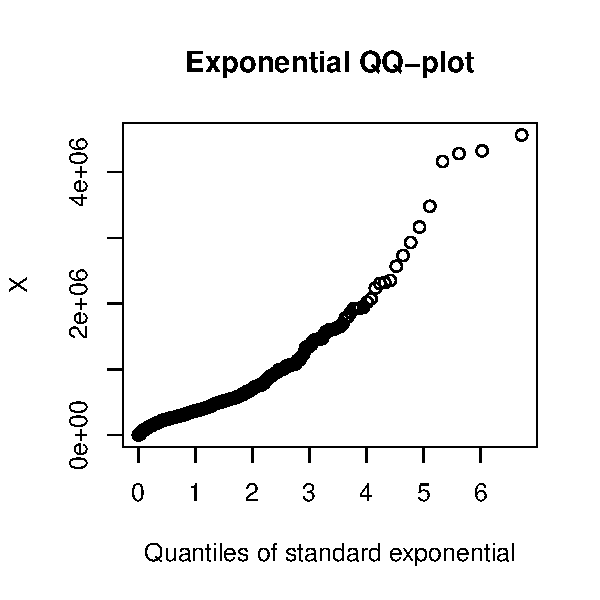
\includegraphics[width=\textwidth]{./plots/ExponentialQQ.pdf}
	\end{subfigure}
	\hfill
	\begin{subfigure}[t]{0.45\textwidth}
		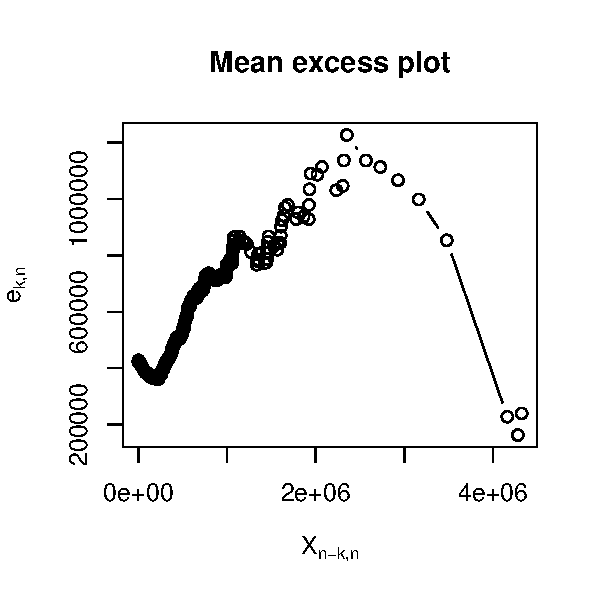
\includegraphics[width=\textwidth]{./plots/MeanExcess.pdf}
	\end{subfigure}
		\begin{subfigure}[t]{0.45\textwidth}
		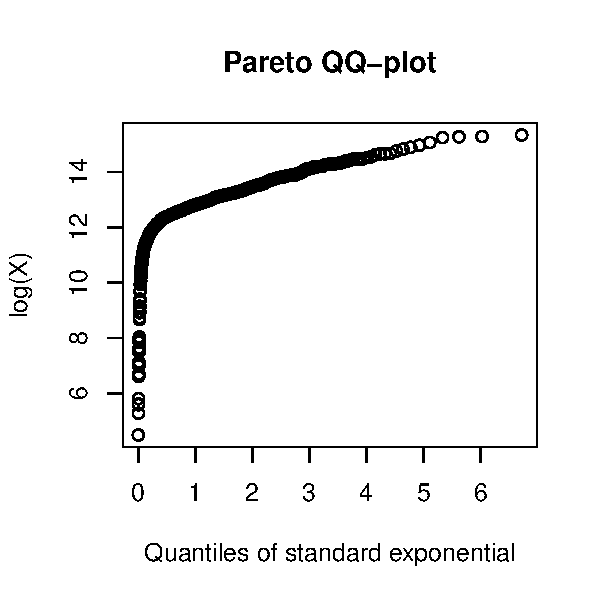
\includegraphics[width=\textwidth]{./plots/ParetoQQ.pdf}
	\end{subfigure}
		\hfill
		\begin{subfigure}[t]{0.45\textwidth}
		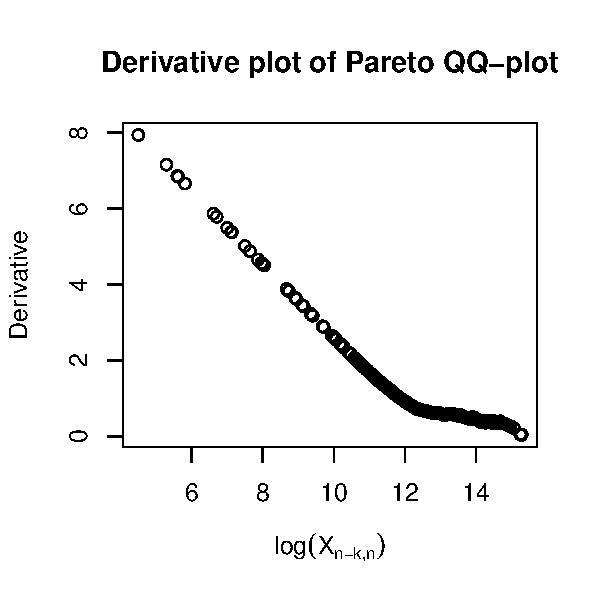
\includegraphics[width=\textwidth]{./plots/ParetoQQ_der.pdf}
	\end{subfigure}
	\caption{Diagnostic plots for the ultimates data}
	\label{diagnostics}
\end{figure}

\newpage
\section{Tail Estimation}
The two most common extreme value approaches for estimating the EVI and corresponding tail quantities thereof are the Block maxima method and the POT method. A short description of these methods are given below. 
\subsection{Block maxima}
The method of block maxima is motivated by the limit behaviour of the normalised maximum as given in (\ref{cond1}), when a non-degenerate distribution exists. The GEV distribution given in (\ref{gev1}), now with the location and scale parameter, can be fitted to the maxima of the sub sample \citep{gumbel1958}

\begin{equation}
G_{\gamma}(x) = 
\begin{cases}
 \exp\left\{ -\left( 1+\gamma\dfrac{x-t}{\sigma} \right)^{-1/\gamma} \right \}, & \text{if}\ \gamma\neq0 \\
 \exp\left\{-\exp\left(\dfrac{x-t}{\sigma} \right) \right\}, & \text{if}\ \gamma=0
\end{cases}
\end{equation}defined on $\{x: 1+\gamma(\dfrac{x-t}{\sigma}) > 0\}$, where $\sigma > 0,\ t \in \mathbb{R}$ and $\gamma \in \mathbb{R}$.

If the IID data are divided into say $m$ blocks then this sub sample consists of the maxima (top observation) extracted from each block. The parameters of the GEV distribution can be estimated either through data analytic methods discussed in \cite{sts626} or using the Maximum likelihood or Probability weighted moment estimators, to name a few.

Corresponding quantile estimates of the GEV can be obtained by inverting the GEV distribution and replacing the parameters ($\gamma,\sigma,t$) with the estimates from and estimation procedure of choice, giving:
\begin{equation}
 z_{p} = 
\begin{cases}
 t - \dfrac{\sigma}{\gamma}\left\{1-[-\log(1-p)]^{-\gamma}\right\}, & \text{if}\ \gamma\neq0 \\
 t - \sigma\log[-\log(1-p)], & \text{if}\ \gamma=0.
\end{cases}
\end{equation}

The block maxima approach suffers some drawbacks. Useful data (extreme values) is discarded in the process of extracting sub samples. Furthermore if block sizes are too small, this can lead to poor asymptotic approximations. Overly large block sizes lead to fewer observations available for inference thus leading to a high variability in the estimates.

One of the ways to overcome this drawback is to model all the data above a sufficiently high threshold. This method is known as the POT approach.

\subsection{Peaks over threshold approach}\label{peaksoverthreshold}
Consider the sequence of IID random variables $X_1,X_2,...,X_n$, the distribution of conditional excesses $Y=X-t$ above a suitably high threshold $t$ is given by:
\begin{equation}\label{conditional}
F_t(y) = P(X-t\leq y|X>t) = \dfrac{F(y+t)-F(t)}{1-F(t)}.
\end{equation}\cite{pickands1975statistical} showed that for any given function $F$ under (\ref{cond1}), the generalised Pareto distribution (GPD) arises as the limit distribution of $F_t(y)$ as $t\rightarrow\infty$.
The distribution function of the GPD is given by:

\begin{equation}\label{gpd}
 G_{\gamma,\sigma_t,t} = 
\begin{cases}
 1-\left\{1+\gamma\left(\dfrac{x-t}{\sigma_t}\right)\right\}^{-1/\gamma}, & \text{if}\ \gamma\neq0 \\
 1 - \exp\left\{-\dfrac{x-t}{\sigma_t}\right\}, & \text{if}\ \gamma=0
\end{cases}
\end{equation}where $x>t,\ \sigma_t >0,\ \left\{1+\gamma\left(\dfrac{x-t}{\sigma_t}\right)\right\} > 0$. The scaling parameter $\sigma_t$ is dependent on $t$ and the GPD shape parameter is the same as the GEV shape parameter. Retrospectively: the GPD appears as the limiting distribution for scaled excesses over a high threshold while the GEV describes the limit distribution of the normalised maxima.

There exists numerous methods for estimating the parameters of the GPD. The most commonly used method is the maximum likelihood (ML) method \citep[see][]{smith1987estimating}. \cite{hosking1987parameter} derived a simple method of moments estimate of $\gamma$ which only works for $\gamma < 0.5$. \cite{castillo1997fitting} further proposed an elemental percentile method which does not impose the $\gamma < 0.5$ restriction. \cite{coles1996bayesian} proposed the use of Bayesian methods.

The corresponding quantile estimates of the GPD can be obtained by inverting (\ref{gpd}), which yields
\begin{equation}
z_p = t +\sigma_t\dfrac{\left(\dfrac{N_t}{np}\right)^{\gamma}-1}{\gamma}\ \text{for}\ p<\dfrac{N_t}{n}.
\end{equation}

Another approach not baring focus in this thesis is the quantile view which rely on versions of the first order condition in (\ref{cond1}). Examples following this approach include but is not limited to the following:
\begin{itemize}
\item \textbf{Pickands estimator}:
\begin{equation*}
\hat{\gamma}_{P,k} = \dfrac{1}{\log 2}\log \left(\dfrac{X_{n-\ceil{k/4}+1,n}-X_{n-\ceil{k/2}+1,n}}{X_{n-\ceil{k/2}+1,n}-X_{n-k+1,n}}\right).
\end{equation*}

\item \textbf{Moment estimator:}
\begin{equation*}
M_{k,n}=H_{k,n} + 1 - \dfrac{1}{2}\left(1-\dfrac{H^2_{k,n}}{H^{(2)}_{k,n}}\right)^{-1}
\end{equation*}where
\begin{equation*}
H^{(2)}_{k,n} = \dfrac{1}{k}\sum^k_{j=1}(\log X_{n-j+1,n} - \log X_{n-k,n})^2.
\end{equation*}

\end{itemize}
It should be noted that in this thesis, the focus is solely placed on improving POT methods.

\subsection{Fitting Pareto type data}
\subsubsection*{Uncensored data}
Pareto tail modelling is the most common approach to modelling large insurance claims. This is because large insurance claims generally exhibit heavy tails. We now focus only on a subset of models for which $\gamma > 0$. 
Indeed if $\gamma>0$ then the tail quantile function is given by \citep{sts626}:
\begin{equation}\label{paretoF}
\bar{F}(x)=x^{-1/\gamma}\ell_F(x)\ \ x\uparrow \infty
\end{equation}where $\ell_F(x)$ is a slowly varying function. This statement is equivalent to 
\begin{equation}\label{paretohill}
\dfrac{\bar{F}(ty)}{\bar{F}(t)}=P\left( \dfrac{X}{t} > y| X > t \right)\rightarrow y^{-1/\gamma},\ t\uparrow \infty
\end{equation}and bares resemblance to (\ref{conditional}) which was stated in terms of the additive (or absolute) excesses $X-t$. For Pareto type data it becomes much more convenient to work with multiplicative excesses $X/t$.

Let the ultimates be IID random variables $X_1,...,X_n$. Equation (\ref{paretohill}) can be used to retrieve the \cite{hill1975simple} estimator, based on the POT approach, by fitting a strict Pareto distribution to the relative excesses using maximum likelihood.

\begin{figure}[t!] 
\centering
	\begin{subfigure}[t]{0.45\textwidth}
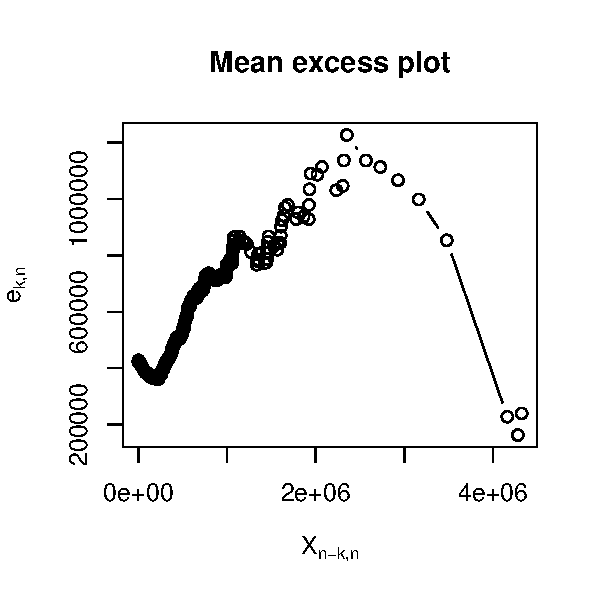
\includegraphics[width=\textwidth]{./plots/MeanExcess.pdf}
	\end{subfigure}
		\begin{subfigure}[t]{0.45\textwidth}
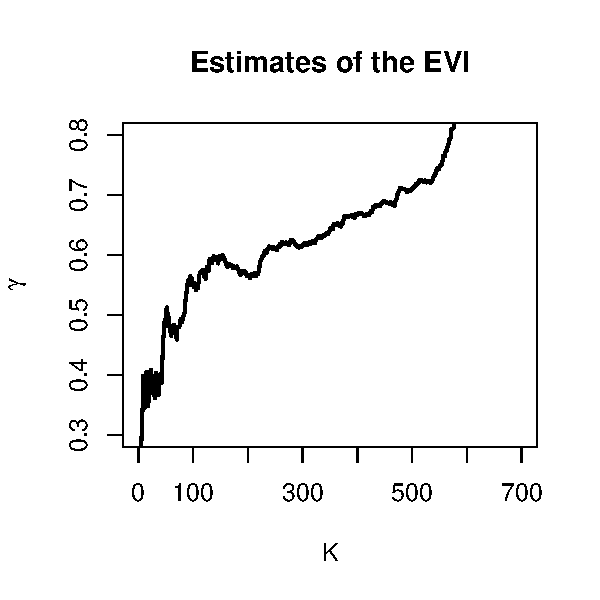
\includegraphics[width=\textwidth]{./plots/HillGPD.pdf}
	\end{subfigure}
	\caption{Mean Excess (left) and Hill estimates of the EVI (right) of the ultimates}
	\label{fig_hillgpd}
\end{figure}
It can be seen from Figure \ref{fig_hillgpd} (right) that the $e_{k,n}$ increases with increasing $X_{n-k,n}$, indicating that the tail of the ultimates data is heavier than exponential and thus validating the use of an estimator of a positive $\gamma$ such as the Hill estimator. Figure \ref{fig_hillgpd} (right) shows a plot of the Hill estimates for the ultimates data as a function of the $k$ (number of observations above the threshold). The plot has no apparent form of stability. This problem is very common in practice where the Hill estimator is volatile and hard to interpret and hence commonly referred to as the \textbf{``Hill horror plot''}. Although there are numerous methods to aid a practitioner in making a suitable choice of the right value of $k$. This choice however is to some degree, subjective. This is further discussed in Section {\ref{thresholdsection}}.

\subsubsection*{Censored data}
One of many difficulties related to tail estimation in EVT is modelling data that is subject to random right censorship. This problem is very common in areas such as reinsurance and survival analysis in clinical trials. 

\textbf{Clinical trials}: suppose for example a study is conducted to see how long patients can survive when placed on a certain drug. At the end of the study, some of these patients may still be alive. This is an example of right censoring. The quantity in question (time to death) is not fully observable. \cite{gomes2011estimation} conducted such a case study to survival data sets.

\textbf{Insurance}: here we can revisit the MTPL data studied in \autoref{mtplsection}. We have discussed the ultimate loss projections made by experts. This data set also contains indexed total incurred values as well as the indexed total paid values.

Figure \ref{mtpl_fourclaims} \footnote{Figure \ref{mtpl_fourclaims} is taken from \cite{albrecher2017reinsurance} with authorisation from the authors} illustrates the development of four claims occurring 1995, 1996, 1997 and 1998. The full line indicates the cumulative indexed payment, while the dashed lines indicates the indexed incurred values. 

The incurred values at a particular point in time are the sum of the already paid amounts and the amounts reserved as estimated by experts. When the two lines meet i.e. the cumulative payment and the incurred value are equal, and the claim is closed. 

This happens in the first and third claim while the second and fourth claim appear to still be in development. These two claims (second and fourth claim) are thus right censored at the time of evaluation (end of 2010). 

\begin{figure}[t]
\centering
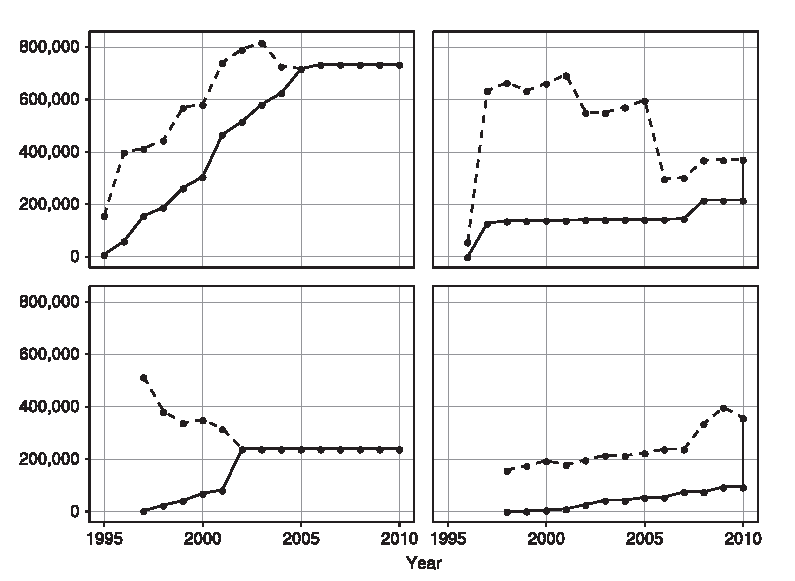
\includegraphics[width=\textwidth]{./plots/mtpl_claims.pdf}
\caption{Development patterns for four particular claims }

\label{mtpl_fourclaims}
\end{figure}
%Figure \ref{mtpl_iti} and Figure \ref{mtpl_itp} shows the indexed total incurred values and total paid values %respectively. As can be expected, most claims occurring closer to 2010 are not developed at the time of %evaluation. 
There will be an inevitable amount of uncertainty in the approximation of ultimate loss projections. Instead of relying on these ultimate loss projections when modelling tail behaviour we can adopt a right censoring framework and only use the indexed total payments at the end of the evaluation year as lower bounds.

Consider $X =\text{\it index total incurred}$ and $C =\text{\it indexed total paid}$. 
We shall work with observations $Z = \min(X,C)$.
\begin{itemize}
\item If a claim is closed at portfolio evaluation then $Z=X$ is observable and the censoring indicator $\Delta = 1$;
\item If a claim is still under development at portfolio evaluation then $Z=C$, thus not completely observable and the censoring indicator $\Delta = 0$;
\end{itemize}Therefore $Z\leq X$ and we use the ordered sample $\{Z_{i,n},\Delta_{i,n},\ i=1,...,n\}$.
This case study is conducted with more detail in \autoref{chap4::Sec6}.
%\begin{figure}[h]
%\centering
%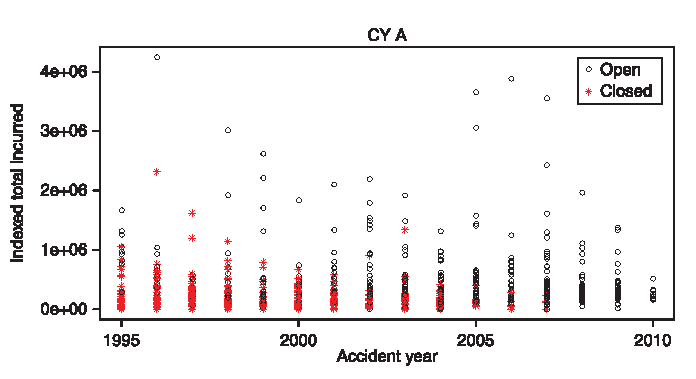
\includegraphics[width=0.95\textwidth]{./plots/ITI.pdf}
%\caption{Company A: incurred losses}
%\label{mtpl_iti}
%\end{figure}

%\begin{figure}[h]
%\centering
%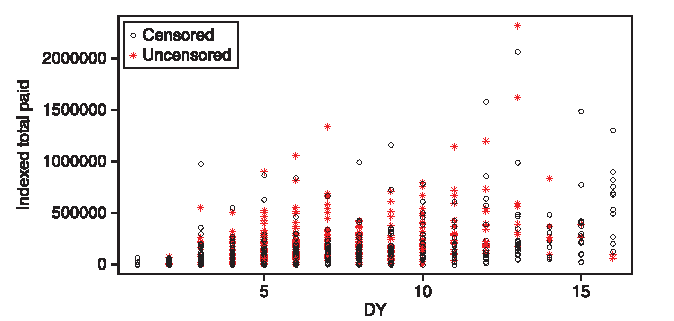
\includegraphics[width=\textwidth]{./plots/ITP.pdf}
%\caption{Company A: incurred losses}
%\label{mtpl_itp}
%\end{figure}

Over the last couple of years, EVT under random right censoring has received considerable attention in literature. A good overview of the subject was made by \cite{beirlant2001pareto} who proposed adapting the Hill estimator under random right censorship.
\\\\
Under some conditions \cite{delafosse2002almost} were able to prove almost sure convergence of this adapted Hill estimator under random right censorship. The authors \cite*{reiss2007statistical} proposed a POT framework by adapting the likelihood function of the distribution of excesses above a threshold. However, the authors did not study the asymptotic properties of the proposed estimators.
\\\\
\cite{beirlant2007estimation} proposed a different approach, generalisation of the POT methodology using the GPD. They also proposed an adaptation of the moment estimator developed by \cite{dekkers1989moment}.
\\\\
\cite{einmahl2008statistics} considered a general adaptation of various estimators of the EVI under random censorship. Under some restrictive conditions, the authors proved the asymptotic normality result of the estimators in detail. \cite{brahimi2015gaussian} proved the asymptotic normality result of the adapted Hill estimator under more relaxed conditions.
\\\\
\cite{gomes2011estimation} provided a good overview of the EVI estimators under random censoring and proposed an adapted minimum-variance reduced-bias (MVRB) estimator \citep{caeiro2005direct}. Using samples from models in the Fréchet domain the authors conducted a simulation study which demonstrated the overall best performance of their adapted MVRB estimator.
\\\\
\cite{worms2014new} presented a methodological paper for the estimation of the EVI under random right censorship, based on the ideas of Kaplan-Meier integration and the synthetic data approach of \cite{sue1987linear}. We show in this thesis how to reinterpret their approach using the mean excess function. Under mild censoring, the authors were able to prove consistency of the proposed estimators.
\\\\
\cite{ameraoui2016bayesian} proposed a Bayesian method to estimate the EVI under random right censoring by developing maximum a posteriori and mean posterior estimators using the Maximal Data Information (MDI), Jeffreys and the conjugate Gamma priors. The authors also establish consistency and asymptotic normality of the proposed estimators.
\\\\
In this thesis a bias reduced version of the \cite{worms2014new} estimator is proposed in \autoref{chap4}, and the idea of shrinkage introduced in \autoref{chap3} is further applied to the proposed estimator. \cite{beirlant2018estimation} study the asymptotic and finite sample behaviour of the large class of estimators first proposed in \cite{worms2014new}, paying special attention to heavy censoring.
\\\\
\subsection{Threshold selection}\label{thresholdsection}
An important question in practical applications of statistics of extremes is the threshold choice. There exists a number of methods available for practitioners to aid in choosing a suitable threshold. The threshold selection problem is however still an open research question. The threshold selection problem is a bias-variance trade off problem \citep{coles2001introduction}. By counterpoint, if the threshold is too high it will lead to fewer excesses to estimate the parameters and will thus lead to a high variance. However if the threshold is too low, the asymptotic motivation of the underlying POT model no longer holds and thus a large bias will be present.
\\\\
The fixed threshold approach is very common in EVT tail estimation. In this approach, the threshold is chosen prior to model fitting. The threshold choice is hereon interchangeably mentioned as; the threshold value from which to consider the data as extremes or the choice of the number ($k$) of upper extremes. 
\\\\
\cite{dumouchel1983estimating} proposed a simple quantity based rule of thumb to consider the top 10\% largest observations as the tail fraction. \cite{loretan1994testing} proposed a data driven approach to choose $k=\dfrac{n^{2/3}}{\log[\log(n)]}$. \cite{ferreira2003optimising} proposed to choose the tail fraction as $k=\sqrt{n}$ through simulation studies. 
\\\\
\cite{hall}, \cite{dekkers1993optimal} and \cite{de1998comparison} proposed choosing a $k$ that minimizes the asymptotic MSE of any proposed estimator. \cite{beirlant1999tail} introduced a heuristically motivated procedure by directly estimating the asymptotic mean squared error. \cite{drees1998selecting} proposed a sequential approach to selecting the optimal sample fraction. Their approach requires an arbitrary choice of a tuning parameter. \cite{draisma1999bootstrap}, \cite{gomes2001bootstrap} and \cite{danielsson2001using} used bootstrap methods to choose the optimal sample fraction. \cite{matthys2000adaptive} provide a review of several adaptive threshold selection techniques. See also Section 4.7 in \cite{sts626}.
\\\\
\cite{dupuis1999exceedances} proposes a method of threshold estimation for the GPD. The procedure assigns to each observation a weight between zero and one. A high weight indicates a good fit and thus the data point should be retained. The author suggests starting with a lower choice of the threshold and increasing it until the weights are all `close to one'. \cite{coles2001introduction} show that diagnostic plots such as the QQ plot, parameter stability plot and the mean excess plot can be used to choose the threshold. Refer to \cite{caeiro2015threshold} for a recent review on the subject of threshold selection.
\\\\
A concern with using the fixed threshold approach is that the threshold value consistent with GPD assumptions is regarded as known and extrapolation is then conducted given this known value. Thus threshold uncertainty is not naturally taken into account. Moreover, in comparing the estimation results from different thresholds, it is often found that plausible but different threshold values, lead to different EVI estimates.

\subsection{Bias reduction}
In order to address the inadequacies of threshold selection under the POT framework, the concept of bias reduction has been studied extensively. Many of these studies however are focused mainly on the $\gamma>0$ case.
\\\\
\cite{peng1998asymptotically}, \cite{caeiro2002class}, \citet{gomesa2002asymptotically,gomes2004bias} and \citet{gomes2002semi,gomes2005revisiting} proposed bias reduction methods that seek to cancel out the bias terms through an indirect approach of using weighted combinations of different estimators.
\\\\
\citet{beirlant1999tail, beirlant2008improved}, \citet{feuerverger1999estimating} and \citet{gomes2000alternatives,gomes2007improving} proposed bias reduction methods based on scaled log-spacings between subsequent high order statistics from a Pareto-type distribution.
\\\\
\cite{caeiro2005direct} proposed minimum variance reduced bias estimators of the EVI, where the bias is reduced without increasing the variance with respect to the Hill estimator. This method is based on adequate external estimation of a pair of parameters of second order slow variation under a third order condition which we do not discuss in this thesis. Following this work, proposals by \cite{gomes2007sturdy,ivette2007simple}, \cite{gomes2008tail} and \citet{caeiro2008minimum} consider directly subtracting the bias term as given by the asymptotic distribution.
\\\\
\cite{beirlant2009second} proposed a much more flexible model adequately capturing the deviation between the true excess right tail function and the asymptotic Pareto model. This approach substantially reduced bias by considering the Hall-class of Pareto-type models in (\ref{hall}). This approach often leads to much improved results, both in bias and MSE.

\\
\subsection{Mixture modelling in EVT}
The main motivation behind use of mixture models in EVT is to improve flexibility of tail models, which generally only focus on the tail part of the data and not the complete data set. This area of research has over the last decade gained considerable interest. \cite{frigessi2002dynamic} proposed an unsupervised tail estimation technique using a dynamic mixtures of two components with a weight function $\pi=\pi(x)$ smoothly connecting the bulk and the tail of the distribution. \cite{sts626} suggested the need for a global statistical model describing the entire range of possible claim outcomes using an exponential and a Pareto mixture.
\\
\cite{behrens2004bayesian} considered a Bayesian approach of fitting a parametric mixture model using indirect expert elicited prior distributions. This Bayesian posterior inference does however have a major draw back. Since it treats the prior on the threshold parameter and other parameters as independent, the dependence between the scale and threshold parameters is simply ignored. \cite{tancredi2006accounting} also accounts for threshold uncertainty by estimating the threshold as one of the parameters in the mixture model. 
\\
\cite{carreau2009hybrid2} proposed a hybrid Pareto model by stitching a GPD tail with a normal distribution and setting a continuity constraint on the density and its first derivative. Performance of this method is however poor in practice. Improvement and extension of the performance of this hybrid Pareto model is made by \cite{carreau2009hybrid1}.
\\
\cite{macdonald2011flexible} considered a mixture approach where the bulk of the distribution is estimated by a standard kernel density estimator. Using penultimate theory \cite{wadsworth2012likelihood} account for threshold uncertainty and provide a likelihood ratio testing procedure for the threshold choice.
\\\\
By applying the inverse CDF of the GPD to more richer Beta distributed draws instead of uniform draws, \cite{papastathopoulos2013extended} proposed general extensions to the GPD distribution. Following from this work, \cite{naveau2016modeling} proposed a version of the extended statistical model called the extended generalised Pareto distribution (EGPD) which is in compliance with EVT and allows for a smooth transition between the modal and tail part of the data. Building further from this work, \cite{tencaliec2018flexible} proposed a flexible semiparametric GP modelling approach by estimating the key component of the EGPD class in \cite{naveau2016modeling} using Bernstein polynomials.

\section{Data sets and Software}
In this section, we give a description of all the data sets used in this thesis for practical illustrations. A description of the software used to conduct simulation studies is also given.

\begin{enumerate}
\item \textbf{Secura Belgian Re data}\\
The Secura Belgian Re is studied in \autoref{chap3} as first studied by \cite{sts626}. The data set contains 371 automobile claims larger than or equal to 1,200,000 Euros for the year 1988 to 2001, collected from various insurance companies in Europe. All amounts have been indexed.
\item \textbf{Motor third-party liability (MTPL) data}\\
Details of this data are given in \autoref{mtplsection}. The data set is further studied in \autoref{chap4}.
\item \textbf{Mont-Aigoual station rainfall data}\\
This rain fall data is studied in \autoref{chap5}. The data set was first studied by \cite{carreau2017partitioning} and \cite{tencaliec2018flexible}. It contains daily precipitation of all seasons from the year 1976 to 2015 recorded at the Mont-Aigoual station, south of France.
\end{enumerate}

\subsection*{Software}
All simulations in this thesis were conducted using the \textbf{R} \citep{R} software through a Linux based high performance computing unit. The simulation study conducted in \autoref{chap5} are more extensive and thus resulted in large output data files. To avoid making too many plots, an interactive web application is build using an \textbf{R} package called shiny \citep{shiny} and hosted as a standalone application on the following url: \url{https://phdshinygao.shinyapps.io/ExtendedModels/}. Guidelines regarding usage of the interactive web application are given in Appendix \ref{shiny}.

\section{Chapter conclusion}
In this chapter, an overview of EVT has been given, along with a review of literature leading up to proposals made in this thesis. A motivating data set was used to give a short illustration of the need for EVT, moreover discuss a growing research interest of an EVT framework for dealing with censored extremes. Finally, descriptions of all the data sets and software used in this thesis were given.
\\\\
The next chapter marks the beginning of \autoref{part1} of the thesis which will introduce the method of shrinkage estimation in \autoref{chap3} and propose a bias reduced estimator of the EVI in \autoref{chap4}. \autoref{chap5} in \autoref{part2} of the thesis will propose a novel bias reduction technique in all domains of attraction and an overall conclusion will be made in \autoref{chap6}.
